\documentclass{article}
\usepackage{amsmath}
\usepackage[margin=1in]{geometry}
\usepackage{tikz}
\begin{document}

\title{ELCT 432: Problem Assignment \#5}
\author{Jacob C. Vaught}
\date{10-28-2023}
\maketitle

\section*{Problem \#1 [20 pts]}
Consider a three-state communication where the communication system transmits the letter \(X\), \(Y\), or \(Z\) randomly each time. The probability of transmitting \(X\), \(Y\), and \(Z\) are \(0.2\), \(0.3\), and \(0.5\), respectively. The communication channel erases the transmitted letter, where the erased letter will be shown as \(E\). For example, if \( (X, Y, Y, Z, Z, X) \) is transmitted, \( (X, E, Y, E, Z, E) \) can be received where the second, fourth, and sixth letters are unknown (erased) at the receiver. Assume that the erasure probability is \(0.05\), \(0.10\), and \(0.15\) if the letter is \(X\), \(Y\), and \(Z\).

\subsection*{Solution for Part 1}
To find the probability of observing an erasure at the output, we calculate:

\[
P(\text{Erasure}) = P(X) \times P(\text{Erasure} | X) + P(Y) \times P(\text{Erasure} | Y) + P(Z) \times P(\text{Erasure} | Z)
\]
\[
P(\text{Erasure}) = 0.2 \times 0.05 + 0.3 \times 0.10 + 0.5 \times 0.15 = 0.115
\]

\subsection*{Solution for Part 2}
Assuming 10,000 letters are transmitted, the number of letters likely to be erased is:

\[
\text{Number of erased letters} = P(\text{Erasure}) \times \text{Total number of letters} = 0.115 \times 10000 = 1150
\]

\subsection*{Solution for Part 3}
To find the probability that an erased symbol is \(X\), \(Y\), or \(Z\), we use conditional probability:

\[
P(X | \text{Erasure}) = \frac{P(X) \times P(\text{Erasure} | X)}{P(\text{Erasure})}
\]
\[
P(X | \text{Erasure}) = \frac{0.2 \times 0.05}{0.115} \approx 0.087
\]

\[
P(Y | \text{Erasure}) = \frac{P(Y) \times P(\text{Erasure} | Y)}{P(\text{Erasure})}
\]
\[
P(Y | \text{Erasure}) = \frac{0.3 \times 0.10}{0.115} \approx 0.261
\]

\[
P(Z | \text{Erasure}) = \frac{P(Z) \times P(\text{Erasure} | Z)}{P(\text{Erasure})}
\]
\[
P(Z | \text{Erasure}) = \frac{0.5 \times 0.15}{0.115} \approx 0.652
\]

\newpage
\section*{Problem \#2 [15 pts]}
Assume that you have a communication system that generates a message with a length of three bits, e.g., \((0,1,1)\), at each time and the messages are equiprobable. Assume that you generate a random variable \(X\) based on counting the number of 1s in the message.

\subsection*{Solution for Part 1}
The sample space of \(X\) is \(\{0, 1, 2, 3\}\).

\subsection*{Solution for Part 2}
\begin{figure}[h!]
  \centering
  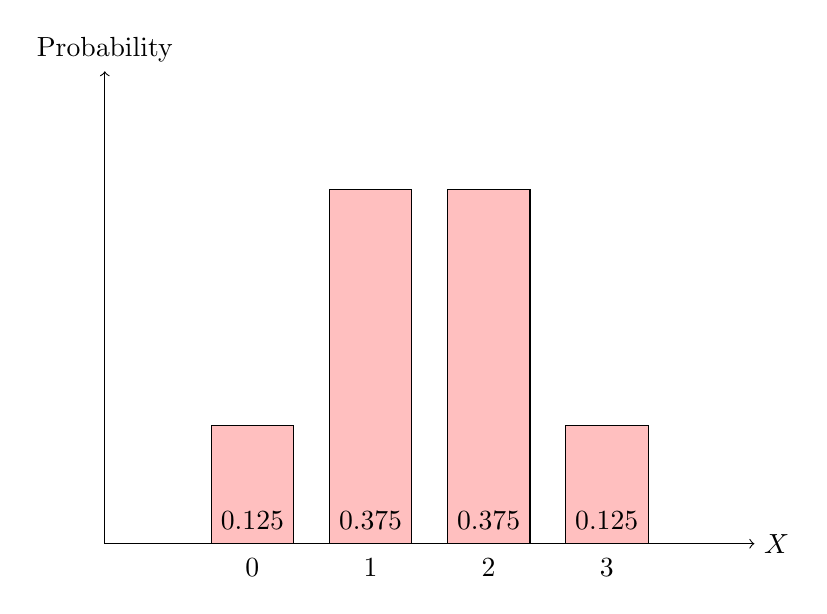
\begin{tikzpicture}[scale=1.5]
    \draw[->] (0,0) -- (5.5,0) node[right] {\(X\)};
    \draw[->] (0,0) -- (0,4) node[above] {Probability};
    \foreach \x/\y in {1/0.125,2/0.375,3/0.375,4/0.125} {
      \draw[fill=pink] (\x-0.1,0) rectangle ++(0.7,\y*8);
      \node at (\x+0.25, 0.2) { \(\y\)};
    }
    \foreach \x/\y in {1/0,2/1,3/2,4/3} {
      \node at (\x+0.25, -0.2) { \(\y\)};
    }
  \end{tikzpicture}
  \caption{PMF of Random Variable \(X\)}
\end{figure}


\subsection*{Solution for Part 3}
\(P(X < 0) = 0\) since the minimum value of \(X\) is 0.

\subsection*{Solution for Part 4}
The probability of \(X\) being less than or equal to 0 can be obtained by considering the case where \(X=0\). There is only one such message, which is \(000\), out of the 8 equiprobable messages. Hence, the probability \(P(X \leq 0)\) is given by:

\[
P(X \leq 0) = P(X=0) = \frac{1}{8}
\]

\subsection*{Solution for Part 5}
The probability of \(X\) being less than or equal to 1 can be obtained by summing the probabilities for \(X=0\) and \(X=1\). For \(X=0\), there is one such message \((000)\), and for \(X=1\), there are three such messages \((001, 010, 100)\). Each message is equiprobable with a probability of \(\frac{1}{8}\). Hence, the probability \(P(X \leq 1)\) is given by:

\[
P(X \leq 1) = P(X=0) + P(X=1) = \frac{1}{8} + \frac{3}{8} = \frac{4}{8} = \frac{1}{2}
\]


\subsection*{Solution for Part 6}
\(P(X > 5) = 0\) since the maximum value of \(X\) is 3.

\subsection*{Solution for Part 7}
\begin{figure}[h!]
  \centering
  \begin{tikzpicture}[scale=1.5]
    \draw[->] (0,0) -- (6,0) node[right, font=\small] {\(X\)};
    \draw[->] (0,0) -- (0,6) node[above, font=\small] {Probability};
    \draw[thick] (1,0.625) -- (2,0.625);
    \draw[thick] (2,2.5) -- (3,2.5);
    \draw[thick] (3,4.375) -- (4,4.375);
    \draw[thick] (4,5) -- (5,5);
    
    \foreach \x/\y in {1/0.125, 2/0.5, 3/0.875, 4/1} {
      \fill (\x,\y*5) circle [radius=0.07];
      \node[align=center, below, font=\small] at (\x, \y*5-0.1) {\(\y\)};
    }
    
    \foreach \x/\y in {1/0, 2/1, 3/2, 4/3, 5/4} {
      \node[align=center, below, font=\small] at (\x, -0.1) {\(\y\)};
    }
  \end{tikzpicture}
  \caption{CDF of Random Variable \(X\)}
\end{figure}


\newpage
\section*{Problem \# 3[15 pts]}
Consider a random binary vector of length \(N\), with equiprobable elements (i.e., 0.5 for bit 0 and 0.5 for bit 1).

\subsection*{Solution for Part 1}
The number of elements in the sample space is \(2^N\).

\subsection*{Solution for Part 2}
The probability of observing an arbitrary binary vector of length \(N\) is \(\left(\frac{1}{2}\right)^N\).

\subsection*{Solution for Part 3}
The probability of observing at least \(0 \leq M \leq N\) elements in the binary vector to be 1 is:

\[
\sum_{M=0}^{N} \binom{N}{M} \left(\frac{1}{2}\right)^N = 1
\]
\newpage
\section*{Problem \# 4[10 pts]}
The signal power of random variable \(X\) can be calculated as \(E(X^2)\), where \(E(X) \triangleq \int x f_X(x) dx\) from \(-\infty\) to \(+\infty\) is the expectation operator. Assume that the mean of the random variable \(X\) is 2 and the standard deviation of \(X\) is 3.

\subsection*{Solution}
To find the signal power \(E(X^2)\), we use the formula:

\[
E(X^2) = \sigma^2 + \mu^2
\]

Given \( \mu = 2 \) and \( \sigma = 3 \):

\[
E(X^2) = 3^2 + 2^2 = 9 + 4 = 13
\]

So, the signal power is 13.
\newpage
\section*{Problem \# 5[10 pts]}
Assume that random variable \(X \sim \mathcal{N}(\mu, \sigma^2)\), where \(\mathcal{N}(\mu, \sigma^2)\) denotes a Gaussian random variable with the variance \(\sigma^2\) and \(\mu\). Which signal is more powerful? Why?

\subsection*{Solution}
Signal power is calculated using the equation \(E(X^2) = \sigma^2 + \mu^2\).

For Signal A with \(\mu = -3\) and \(\sigma^2 = 1\):
\[
E_A(X^2) = (-3)^2 + 1 = 10
\]

For Signal B with \(\mu = 3\) and \(\sigma^2 = 1\):
\[
E_B(X^2) = (3)^2 + 1 = 10
\]

For Signal C with \(\mu = 0\) and \(\sigma^2 = 5\):
\[
E_C(X^2) = (0)^2 + 5 = 5
\]

Both Signal A and Signal B have the same power, \(E(X^2) = 10\), which is greater than the power of Signal C, \(E(X^2) = 5\). Therefore, Signal A and Signal B are more powerful than Signal C.
\newpage

\section*{Problem \# 6[30 pts]}

Assume that you have \(N\) i.i.d. (independent and identically distributed) random variable with a uniform PDF between 0 and \(L\). However, you don't know the value of \(L\). You try to estimate the value of \(L\) as \(L' = \max\{X_1, X_2, \ldots, X_N\}\), where \(X_k \sim U[0, L]\) denotes the \(k\)-th random variable.

\subsection*{Solution for Part 1}

To find the PDF (Probability Density Function) of \(L'\), first consider its CDF \(F_{L'}(x)\):

\[
F_{L'}(x) = P(L' \leq x) = P(X_1 \leq x, X_2 \leq x, \ldots, X_N \leq x) = \left(\frac{x}{L}\right)^N
\]
Differentiating \(F_{L'}(x)\) with respect to \(x\), we get:

\[
f_{L'}(x) = \frac{d}{dx} \left(\frac{x}{L}\right)^N = \frac{N}{L} \left(\frac{x}{L}\right)^{N-1}
\]
This is valid for \(0 \leq x \leq L\).

\subsection*{Solution for Part 2}
The expected value of \(L'\) is:

\[
E[L'] = \int_{0}^{L} x f_{L'}(x) dx = \frac{N}{N+1}L
\]
The expected value of the error \(E[L' - L]\) is:

\[
E[L' - L] = E[L'] - L = \frac{N}{N+1}L - L = -\frac{L}{N+1}
\]
\end{document}